\tikzset{lien/.style={->,>=latex,rounded corners=5pt}}
\tikzset{individu/.style={draw,fill=#1!25},individu/.default={green}}

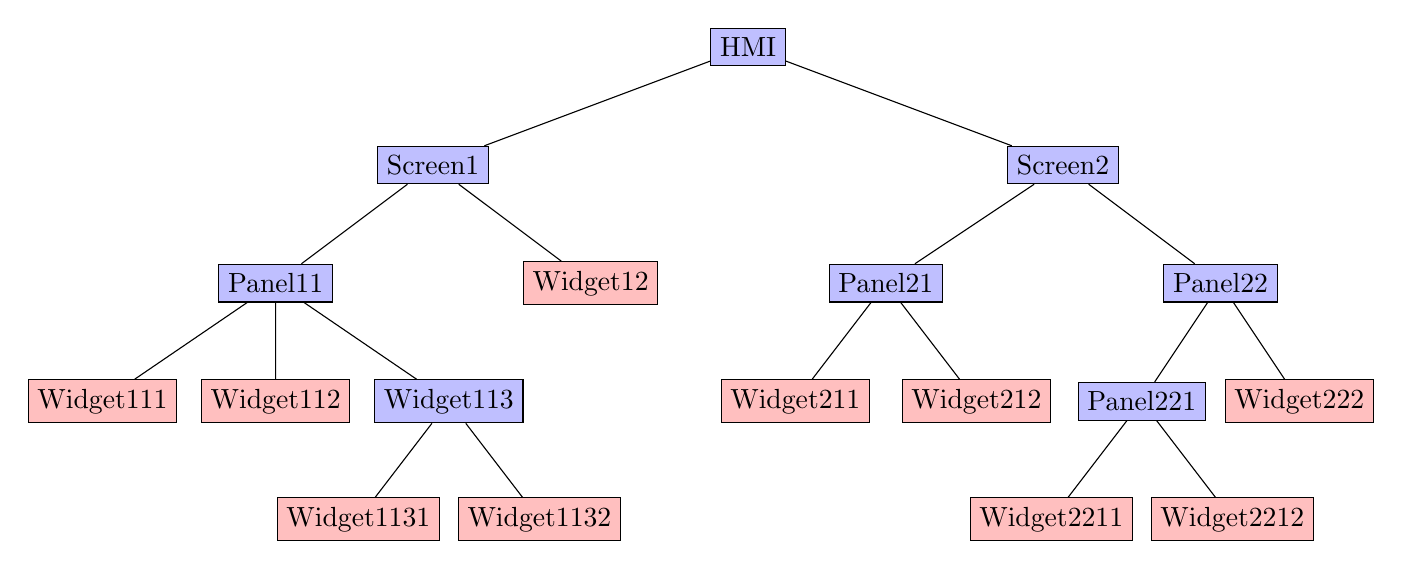
\begin{tikzpicture}
[level 1/.style={sibling distance=8cm},
level 2/.style={sibling distance=4cm},
level 3/.style={sibling distance=2cm}]
\node [individu=blue] {HMI}
child{ node [individu=blue]{Screen1}
	child  { node [individu=blue]{Panel11} 
		child [sibling distance=2.2cm] { node [individu=red] {Widget111} }
		child [sibling distance=2.2cm] { node [individu=red] {Widget112} }
		child [sibling distance=2.2cm] { node [individu=blue] {Widget113} 
			child [sibling distance=2.3cm] { node [individu=red] {Widget1131} }
			child [sibling distance=2.3cm] { node [individu=red] {Widget1132} }
		}
	}
	child { node [individu=red]{Widget12} }
}
child{ node [individu=blue]{Screen2}
	child  [sibling distance=4.5cm] { node [individu=blue]{Panel21} 
		child [sibling distance=2.3cm]{ node [individu=red]{Widget211} }
		child [sibling distance=2.3cm]{ node [individu=red]{Widget212} }
	}
	child { node [individu=blue]{Panel22}
		child { node [individu=blue]{Panel221} 
			child [sibling distance=2.3cm]{ node [individu=red]{Widget2211} }
			child [sibling distance=2.3cm]{ node [individu=red]{Widget2212} }
		}
		child { node [individu=red]{Widget222} } 
	}
};
\end{tikzpicture}

